 \documentclass{article}
    \usepackage{amsmath}
    \usepackage[utf8]{inputenc}
    \usepackage[english]{babel}
    \usepackage{color}
    \usepackage{graphicx}
    \usepackage{enumitem}
    \usepackage{incgraph}
    \hyphenpenalty=10000
    \exhyphenpenalty=10000
    % \usepackage[T1]{fontenc}
    % \usepackage{geometry}
    \usepackage[top = 2cm, bottom = 2cm]{geometry}
    
    \usepackage[familydefault,light]{Chivo} 
    \usepackage[T1]{fontenc}
    
    \setlength{\parindent}{4em}
    \setlength{\parskip}{2em}
\renewcommand{\baselinestretch}{1.5}
    \usepackage{graphicx}
    
    \title{COL 783 \\ Assignment 3}
    \author{Rajbir Malik \\ 2017CS10416}
    
    \begin{document}
    
    \maketitle

%  Starting page
% -------------------------------------------------------
% -------------------------------------------------------
    \begin{center}
    \Large{\underline{\textbf{Pyramids and Wavelets}}}
    \end{center}
    \subsection*{Overview}
    In this assignment, we tried various transforms and transformations on the images, checking their benifits in \textit{denoising} and \textit{compression}.\\ 
    We worked with pyramids, \textit{laplacian} and \textit{gaussian}, we tried blending of images based on paper by \textbf{Burt and Adelson (1983)}. We, also, used pyramids to denoise various images.\\
    We then worked on \texttt{Haar Transform} and \texttt{Lazy-Lifting Transform}, and used them for denoising and compression. I deviced my own encoding and decoding schemes, which seemed to suit very well.\\
    I also implemented one of the bonus exercises, the one involving lazy lifting-scheme based transform.
% -------------------------------------------------------
% -------------------------------------------------------
% Topic I
    \pagebreak
    \subsection*{Image Blending Using Pyramids}
% -------------------------------------------------------
    The pyramid based blending was introduced by \textit{Burt and Adelson (1983)}, which allowed seamless merging of images using their pyramids.\\
    
    \textbf{Example}\\
% -------------------------------------------------------

    \begin{figure}[!htb]
    %
    \minipage{0.33\textwidth}
    \begin{center}
      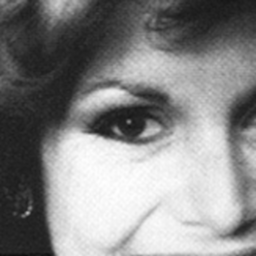
\includegraphics[scale=.55]{./blending/eh/face.png}
      \caption{Face}
    \end{center}
    \endminipage \hfill
    %
    \minipage{0.33\textwidth}
    \begin{center}
      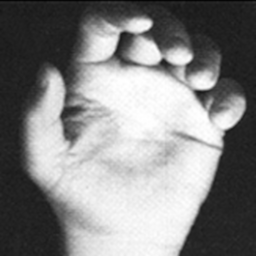
\includegraphics[scale=.55]{./blending/eh/hand.png}
      \caption{Hand}
     \end{center}
    \endminipage \hfill
    %
    \minipage{.33\textwidth}
    \begin{center}
      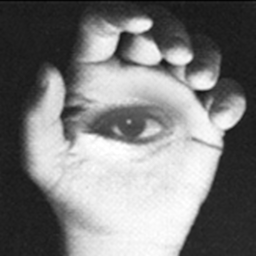
\includegraphics[scale=.55]{./blending/eh/final_1.png}
      \caption{Merge}
    \end{center}
    \endminipage
    \end{figure}
% -------------------------------------------------------    
    \\[5pt]\textbf{Another example}\\
    Here, I've smoothened the merge even further, by using different splines, each increasingly smoother.\\
    This lead to increasing compatibility (or acceptability) of merge.\\[3pt]
% -------------------------------------------------------
    \begin{figure}[!htb]
    %
    \minipage{0.45\textwidth}
    \begin{center}
      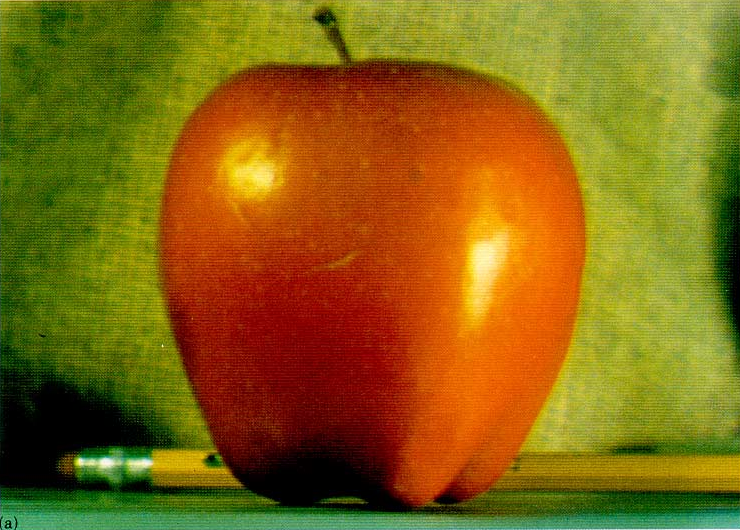
\includegraphics[scale=.35]{./blending/ao/apple.png}
      \caption{Apple}
    \end{center}
    \endminipage \hfill
    %
    \minipage{0.45\textwidth}
    \begin{center}
      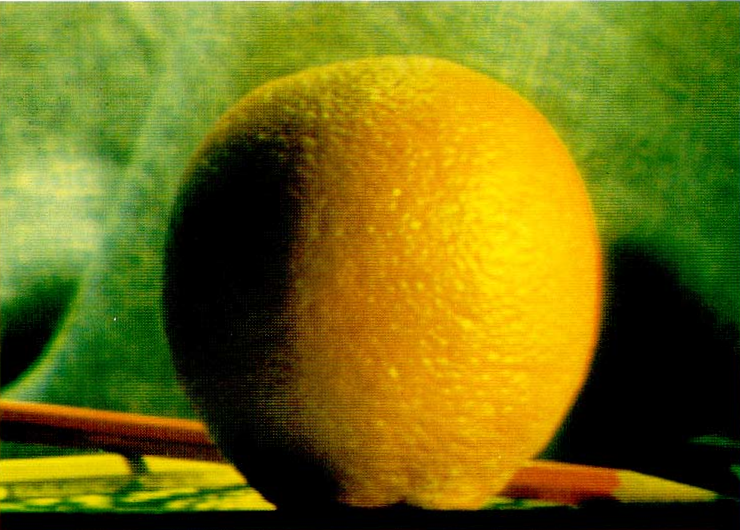
\includegraphics[scale=.35]{./blending/ao/orange.png}
      \caption{Orange}
     \end{center}
    \endminipage \hfill
    %
    \end{figure}

% -------------------------------------------------------
    \pagebreak
% -------------------------------------------------------
    \begin{figure}[!htb]
    \minipage{0.5\textwidth}
      \fbox{
\includegraphics[scale=.25]{./blending/ao/1.png}}
      \caption{Merger}
    \endminipage \hfill
    %
    \minipage{0.5\textwidth}
      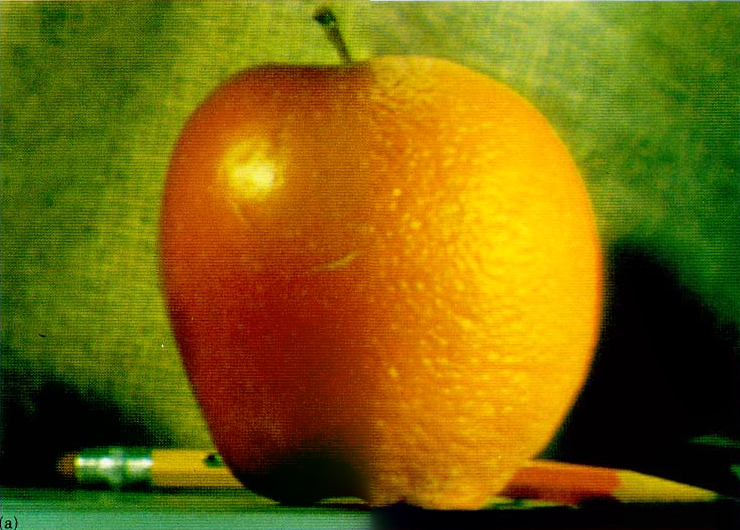
\includegraphics[scale=.3]{./blending/ao/final_1.png}
      \caption{Merge}
    \endminipage \hfill
    %
    \end{figure}

% -------------------------------------------------------
    
    \begin{figure}[!htb]
    \minipage{0.5\textwidth}
      \fbox{
\includegraphics[scale=.25]{./blending/ao/2.png}}
      \caption{Merger}
    \endminipage \hfill
    %
    \minipage{0.5\textwidth}
      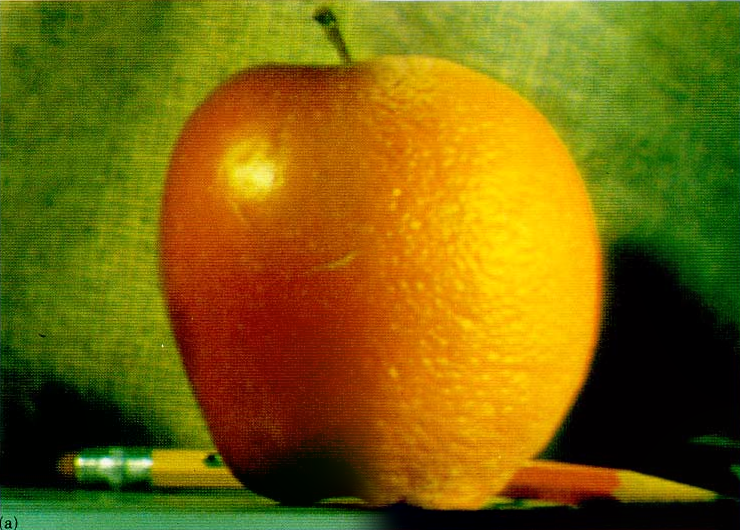
\includegraphics[scale=.3]{./blending/ao/final_2.png}
      \caption{Merge}
    \endminipage \hfill
    %
    \end{figure}

% -------------------------------------------------------
    \begin{figure}[!htb]
    \minipage{0.5\textwidth}
      \fbox{
\includegraphics[scale=.25]{./blending/ao/3.png}}
      \caption{Merger}
    \endminipage \hfill
    %
    \minipage{0.5\textwidth}
      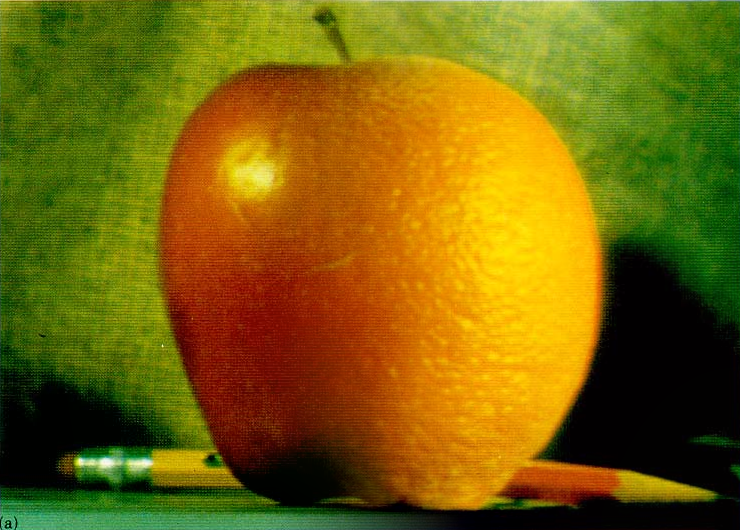
\includegraphics[scale=.3]{./blending/ao/final_3.png}
      \caption{Merge}
    \endminipage \hfill
    %
    \end{figure}
    
    \pagebreak
% -------------------------------------------------------
% Denoising
    \subsection*{Denoising}
    Since noise only adds to the detail of the image (not the approximation), we can very well reduce the noise in the image by working with the detail-levels in transforms and pyramids. Using this idea (usually with coefficient cutoff-thresholding), I tried to denoise some images. Results are presented below.\\[1pt]
    
    \textbf{Image}: Barbara  \textbf{Type}: Continuous (Real World Image)\\

    \begin{figure}[!htb]
    \minipage{0.45\textwidth}
      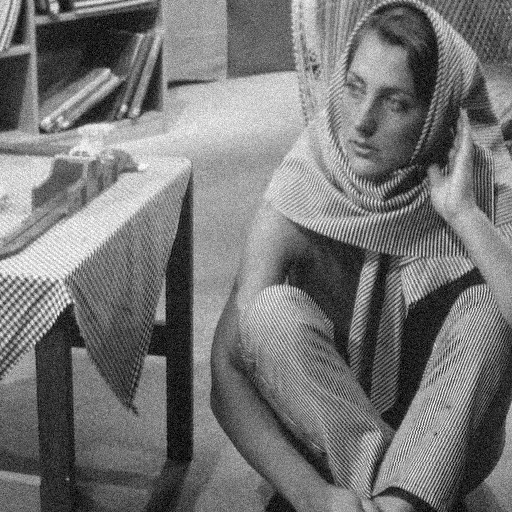
\includegraphics[scale=0.4]{./denoising/b/b05.png}
      \caption{Noisy Image}
    \endminipage \hfill
    \minipage{0.45\textwidth}
      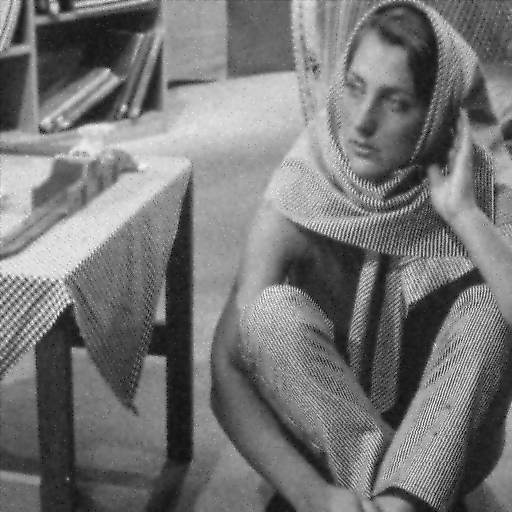
\includegraphics[scale=.4]{./denoising/b/p_1_0_013.png}
      \caption{Pyramid Denoising}
    \endminipage
    \end{figure}\\
    

    \begin{figure}[!htb]
    \minipage{0.45\textwidth}
      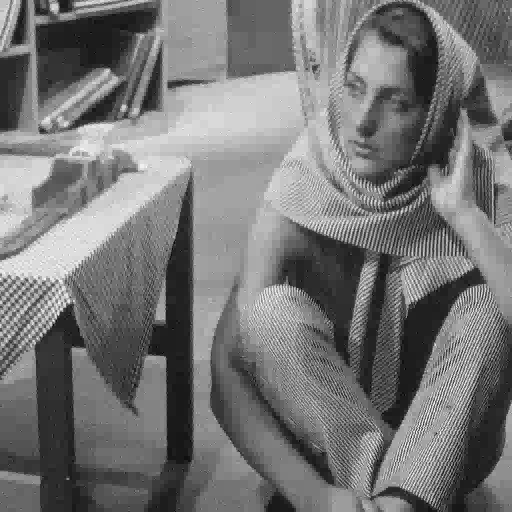
\includegraphics[scale=0.4]{./denoising/b/hard0_15.png}
      \caption{Hard Denoising}
    \endminipage \hfill
    \minipage{0.45\textwidth}
      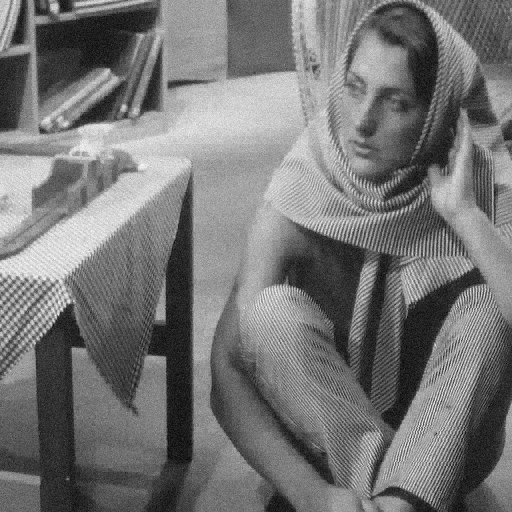
\includegraphics[scale=.4]{./denoising/b/smooth0_05.png}
      \caption{Soft Denoising}
    \endminipage
    \end{figure}
    \pagebreak

%---------------------------------------------
    
    \pagebreak
    \textbf{Image}: Shepplogan  \textbf{Type}: Discrete (Cartoon Image)\\
    
    \begin{figure}[!htb]
    \minipage{0.45\textwidth}
      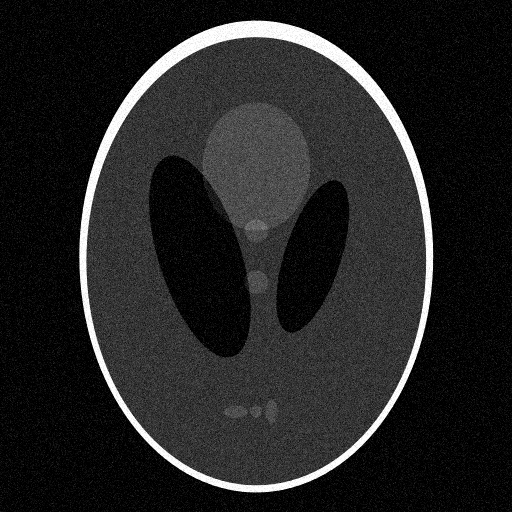
\includegraphics[scale=0.4]{./denoising/n/n05.png}
      \caption{Noisy Image}
    \endminipage \hfill
    \minipage{0.45\textwidth}
      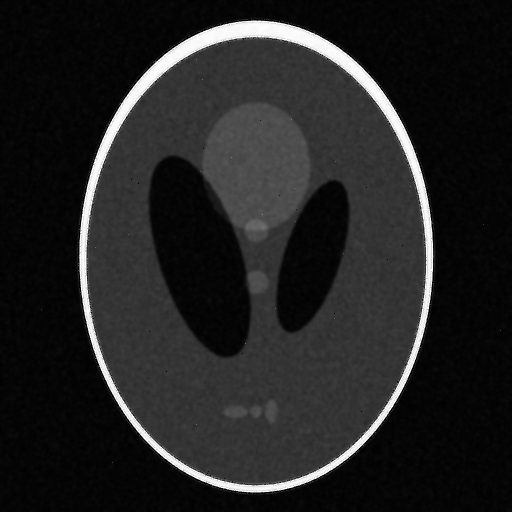
\includegraphics[scale=.4]{./denoising/n/p_1_0_013.png}
      \caption{Pyramid Denoising}
    \endminipage
    \end{figure}
    

    \begin{figure}[!htb]
    \minipage{0.45\textwidth}
      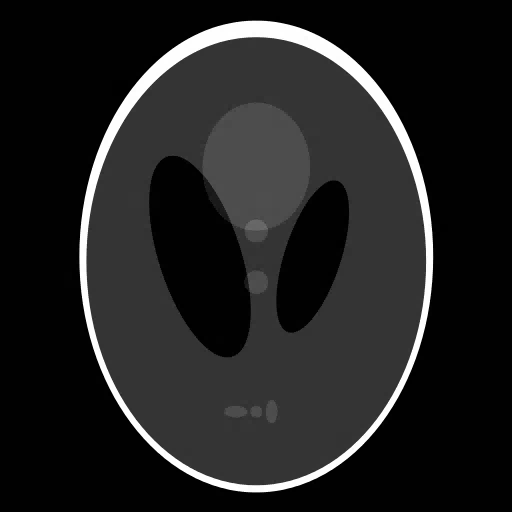
\includegraphics[scale=0.4]{./denoising/n/hard0_05.png}
      \caption{Hard Denoising}
    \endminipage \hfill
    \minipage{0.45\textwidth}
      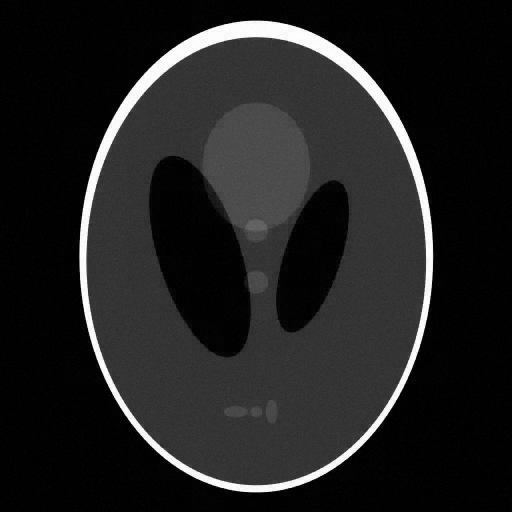
\includegraphics[scale=.4]{./denoising/n/smooth0_05.png}
      \caption{Soft Denoising}
    \endminipage
    \end{figure}
    
    \textbf{Observation}\\
    It was observed that the transform based denoising worked much better than thresholding using laplacian pyramids. Also, denoising worked much better in the case of discrete image, than continuous one. Also, though slight, there was a subtle difference between soft and hard denoising, with soft being more smooth (or acceptable).
    
    
    \pagebreak

%--------------------------------------------- 
% Compression
    \subsection*{Compression}
    We can achieve (lossy) image compression by letting go of smaller detail-coefficients, with thresholding. This allows us to reduce the size, with some sacrifice to the image quality.
    \\Also, we could now encode the image using run-length encoding as detail coefficients are very close to zero, and with cut-off, mostly zero. I tried compression with some images. Results are presented below.\\[2pt]
    \textbf{Image}: Barbara  \textbf{Type}: Continuous (Real World Image)\\
    \begin{figure}[!htb]
    \minipage{0.45\textwidth}
      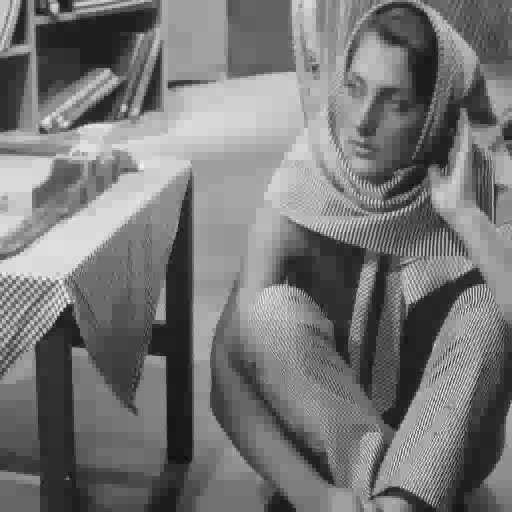
\includegraphics[scale=0.4]{./compression/1/20.png}
      \caption{K = 20, Size = 154KB}
    \endminipage \hfill
    \minipage{0.45\textwidth}
      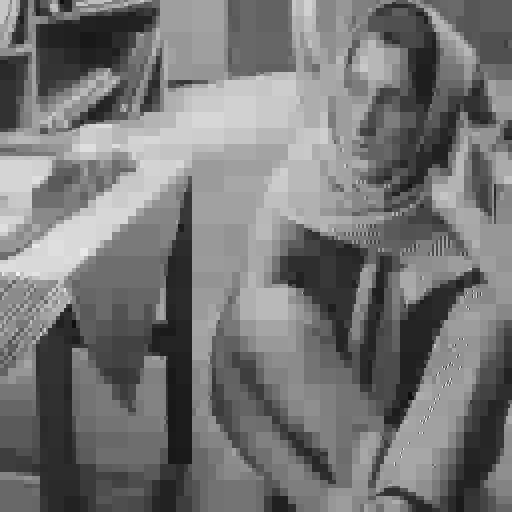
\includegraphics[scale=.4]{./compression/1/50.png}
      \caption{K = 50, Size = 29KB}
    \endminipage
    \end{figure}
    

    \begin{figure}[!htb]
    \minipage{0.45\textwidth}
      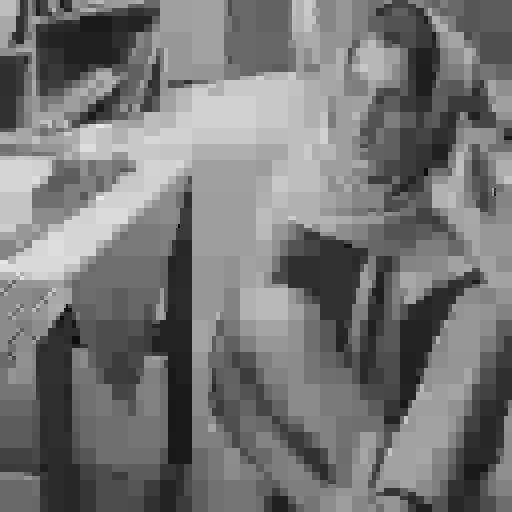
\includegraphics[scale=0.4]{./compression/1/80.png}
      \caption{K = 80, Size = 15KB}
    \endminipage \hfill
    \minipage{0.45\textwidth}
      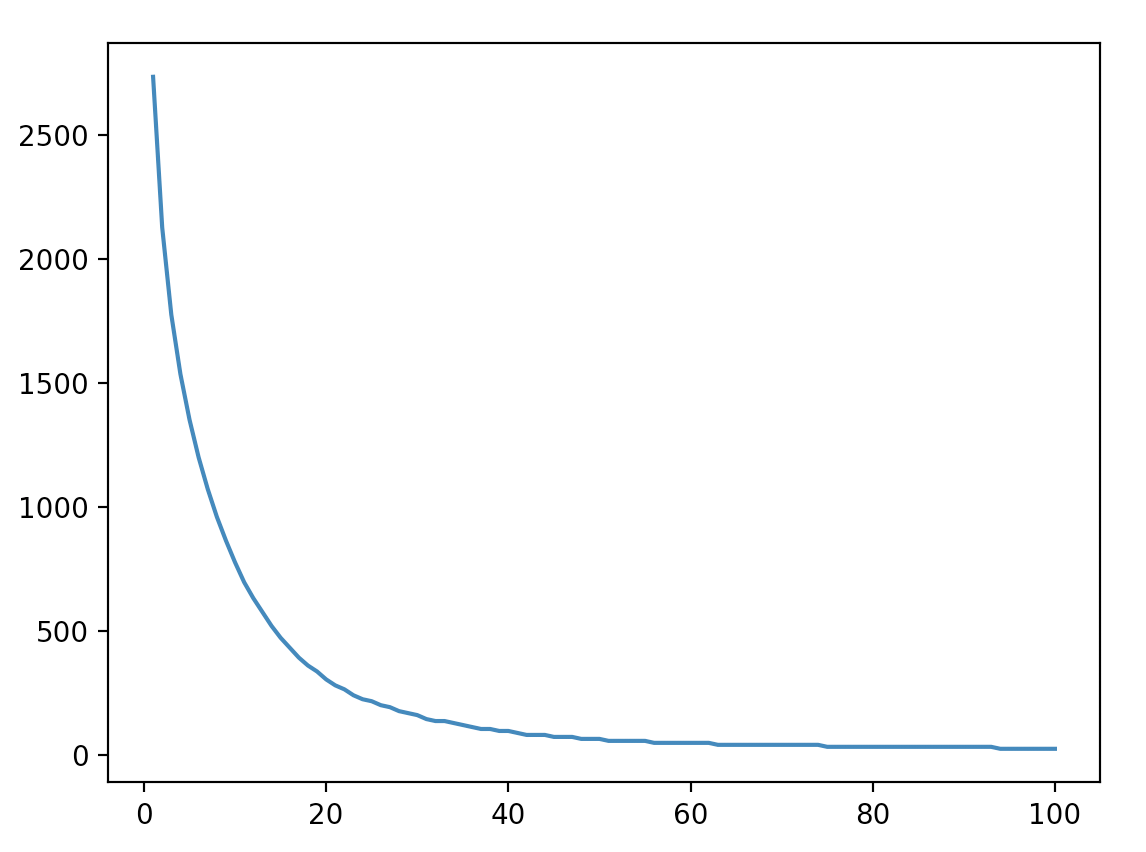
\includegraphics[scale=.4]{./compression/plots/b.png}
      \caption{Plot of binary-size vs. K}
    \endminipage
    \end{figure}
    
%------------------------------------
    \pagebreak
    \textbf{Image}: Shepplogan  \textbf{Type}: Discrete (Cartoon Image)\\
    \begin{figure}[!htb]
    \minipage{0.45\textwidth}
      
\includegraphics[scale=0.4]{./compression/2/20.png}
      \caption{K = 20, Size = 67KB}
    \endminipage \hfill
    \minipage{0.45\textwidth}
      
\includegraphics[scale=.4]{./compression/2/50.png}
      \caption{K = 50, Size = 32KB}
    \endminipage
    \end{figure}
    

    \begin{figure}[!htb]
    \minipage{0.45\textwidth}
      
\includegraphics[scale=0.4]{./compression/2/80.png}
      \caption{K = 80, Size = 18KB}
    \endminipage \hfill
    \minipage{0.45\textwidth}
      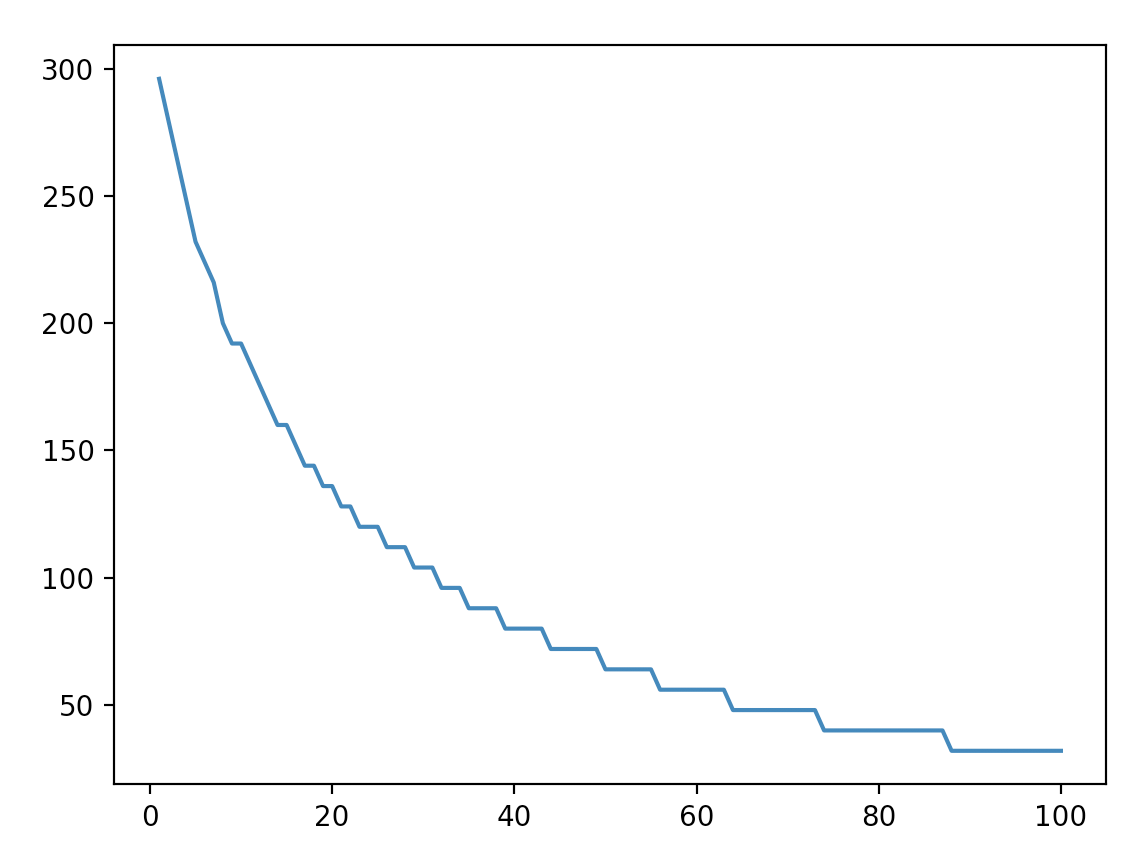
\includegraphics[scale=.4]{./compression/plots/c.png}
      \caption{Plot of binary-size vs. K}
    \endminipage
    \end{figure}

    \textbf{Observation}\\
    I feel, nice compression ratios were achieved :)\\
    Also, it was observed, that in the case of a continuous real world image, the compression increased phenomenally initially, and then slowed down as mostly coarse values remained. In the case of discrete image, instead, the starting value was already very small and the progression in compression was relatively slow, this maybe because most of the detail-coefficients are already small.
    
%--------------------------------------------- 
\pagebreak
%---------------------------------------------
% Bonus
\subsection*{Wavelets with Lifting Scheme}

%--------------------------------------------- 
\pagebreak
%---------------------------------------------
% Summary
\subsection*{Summary}

\end{document}